\usetikzlibrary{arrows,positioning}

\subsection{Configurators in the Wild}

\subsubsection*{Cars}

\begin{frame}{\myframetitle}
	\begin{fancycolumns}[b,widths={67}]
		\begin{exampletight}{Configuring a car \ldots}
			\centering\small%
			\only<1-3>{\pic[width=\linewidth]{toyota-aygo-wheels0}}%
			\only<4-5|handout:0>{\pic[width=\linewidth]{toyota-aygo-wheels}}%
			\only<6-7|handout:0>{\pic[width=\linewidth]{toyota-aygo-wheels2}}%
			\only<8-9|handout:0>{\pic[width=\linewidth]{toyota-aygo-wheels2b}}%
			\only<10|handout:0>{\pic[width=\linewidth]{toyota-aygo-wheels}}%
			\only<11-12|handout:0>{\pic[width=.8\linewidth]{toyota-aygo-color}}%
			\only<13|handout:0>{\pic[width=.8\linewidth]{toyota-aygo-color2}}%
			\only<14-15|handout:0>{\pic[width=\linewidth]{toyota-aygo-wheels3}}%
			\only<16-|handout:0>{\pic[width=\linewidth]{toyota-aygo-wheels4}}%
		\end{exampletight}
	\nextcolumn
		\vspace{-\textheightoftitle}
		\begin{example}{\ldots\ is complicated!}
			\begin{enumerate}
				\item the default configuration
				\uncover<3->{\item we want \textbf{black cap}}
				\uncover<5->{\item we want \textbf{white wheels}}
				\uncover<6->{\item black cap unavailable,\\red selected automatically\\(not blue!)}
				\uncover<7->{\item fine, back to \textbf{black wheels}}
				\uncover<9->{\item and, back to \textbf{black cap}}
				\uncover<11->{\item \textbf{confirm selection} to continue with selection of the car color}
				\uncover<12->{\item we want a \textbf{red car}}
				\uncover<14->{\item popup dialog: black wheels unavailable (no automatic selection! preview of unavailable wheels!)}
			\end{enumerate}
			\uncover<15->{what now? back to Step 3?}
		\end{example}
	\end{fancycolumns}
\end{frame}

\begin{frame}{\myframetitle}
	\begin{fancycolumns}[t,columns=3,widths={33,22}]
		\begin{exampletight}{Configuring a Car \ldots}
			\pic[width=\linewidth]{toyota-aygo-wheels3}\\\centering
			10. cancel the dialog
		\end{exampletight}
	\nextcolumn
		\begin{exampletight}{with a Weird Price}
			\centering\picDark[width=\linewidth]{toyota-aygo-costs}
		\end{exampletight}
	\nextcolumn
		\begin{exampletight}{with 8 Wheels!}
			\picDark[width=\linewidth]{toyota-aygo-costs3}
		\end{exampletight}
	\end{fancycolumns}
	\begin{fancycolumns}[columns=3,widths={20,60},animation=none]
	\nextcolumn
		\uncover<4->{
			\begin{note}{}
				\begin{itemize}
					\item canceling the dialog was not considered and lead to an invalid state (i.e., configuration)
					\item humans check these configurations, but some errors are only found during production
					\item many constraints: appear arbitrary, not explained
				\end{itemize}
			\end{note}
		}
	\nextcolumn
	\end{fancycolumns}
\end{frame}

\begin{frame}{\myframetitle}
	\begin{fancycolumns}[widths={70,30}]
		\begin{exampletight}{Configuring a German Car\mysource{example from \lectureintroduction}}
			\picDark[width=\linewidth]{bmw-series1-confassistant-bluetooth}
		\end{exampletight}
	\nextcolumn
		\begin{note}{}
			Why does the telephone conflict with Microsoft Office?
		\end{note}
	\end{fancycolumns}
\end{frame}

\subsubsection*{Notebooks}

\begin{frame}{\myframetitle}
	\begin{fancycolumns}[widths={65}]
		\begin{exampletight}{Configuring a Notebook} % it is on purpose that both pictures are shown in handout
			\only<1>{\picDark[width=\linewidth]{thinkpad-x1-yoga-display}}
			\only<2->{\picDark[width=\linewidth]{thinkpad-x1-yoga-display-invalidconf}}
		\end{exampletight}
	\nextcolumn
		\begin{note}{}
			can detect mistakes, but provides no explanations or fixes
		\end{note}
	\end{fancycolumns}
\end{frame}

\begin{frame}{\myframetitle}
	\begin{fancycolumns}[widths={70,30}]
		\begin{exampletight}{Still Configuring a Notebook}
			\picDark[width=\linewidth]{thinkpad-x1-yoga-office}
		\end{exampletight}
	\nextcolumn
		\begin{note}{}
			allows some feature combinations and not others, prices are opaque
		\end{note}
	\end{fancycolumns}
\end{frame}

% TODO further example? unclear why certain options are missing: windows10-sign-in-options

% TODO excurs on selectors? amazon-tshirt, ebay-smartphone-case. pictures available, but probably not enough time for that here.

\subsection{Automated Analysis of Feature Models}

\begin{frame}{\myframetitle}
	\begin{fancycolumns}
		\begin{note}{Open Questions}
			\begin{itemize}
				\item How do such configurators work?
				\item How to avoid inconsistencies?
				\item How to provide explanations and fixes? % TODO not explained in this part. remove?
    			\item How to get all valid configurations automatically? (\emph{P2(b)})
			\end{itemize}
		\end{note}
		\begin{definition}{Automated Analysis of Feature Models}
			\begin{itemize}
				\item up until now: \emph{creation} and \emph{transformation} of feature models
				\item now: \emph{analysis} of feature models to improve our understanding of a configuration space
				\item for brevity: product = valid configuration
			\end{itemize}
		\end{definition}
	\nextcolumn
		\begin{example}{Asking Questions About Feature Models}
			\begin{itemize}
				\item Is a given configuration valid?
				\item Is there any product at all?\\
					How many/which products are there?\\
				\item Is a given feature (de-)selectable at all?\\
					How many/which products include it?\\
				\item Is a given partial configuration consistent?\\
					How many/which products include it?\\
				\item \color{gray}{(Which features always occur together?)}
				\item \color{gray}{(Is a given constraint redundant?)}
				\item \color{gray}{(How do two feature model versions differ?)}
				\item \color{gray}{(Why is \ldots? How to fix \ldots?)}
			\end{itemize}
		\end{example}
	\end{fancycolumns}
\end{frame}

\subsection{SAT, \ssat{}, and AllSAT}

\begin{frame}{\myframetitle}
	\begin{fancycolumns}
		\begin{definition}{Recap: Boolean Satisfiability Problem (SAT)}
			\begin{itemize}
				\item \emph{decision problem}: is there any assignment $A$ that satisfies a given formula?
				\item formally: $SAT(\phi) \mequals \exists A \colon \phi(A) = \top$
				\item known to be \emph{NP-complete}:\\
					in theory, difficult to solve if $P \neq NP$;\\
					in practice, solvability depends on domain
				\item answered by \emph{SAT solvers}:\\
					highly-optimized, off-the-shelf tools;\\
					competitively developed over several decades;\\
					takes a CNF in DIMACS format as input
			\end{itemize}
		\end{definition}
		\begin{example}{}
			\begin{itemize}
				\item $X \pimplies Y$ is satisfiable
				\item $X \por \pnot X$ is satisfiable (even a tautology)
				\item $X \pand \pnot X$ is not satisfiable (why?)
			\end{itemize}
		\end{example}
	\nextcolumn
		\begin{definition}{Sharp Satisfiability Problem (\ssat{})}
			\begin{itemize}
				\item \emph{counting problem}: how many assignments satisfy a given formula?
				\item $\ssat(\phi) = \abs{\{A \mid \phi(A) = \top\}}$
				\item known to be \emph{\texttt{\#}P-complete}:\\
					at least as hard as SAT (probably harder)
				\item answered by \emph{\ssat{} solvers}
			\end{itemize}
		\end{definition}
		\uncover<3->{
			\begin{definition}{Solution Enumeration Problem (AllSAT)}
				\begin{itemize}
					\item \emph{enumeration problem}: which assignments satisfy a given formula?
					\item $AllSAT(\phi) = \{A \mid \phi(A) = \top\}$
					\item at least as hard as \ssat{} (probably harder)
					\item answered by \emph{AllSAT solvers}
				\end{itemize}
			\end{definition}
		}
	\end{fancycolumns}
\end{frame}

\begin{frame}{Automated Analysis of Feature Models}
	\begin{fancycolumns}[widths={52}]
		\begin{example}{Asking Questions About Feature Models}
			\begin{itemize}
				\item Is a given configuration valid? $\Rightarrow$ \emph{evaluate}
				\item \emph{Is} there any valid configuration at all?\\
					\emph{How many}/\emph{which} valid configurations are there?\\
				\item \emph{Is} a given feature (de-)selectable at all?\\
					\emph{How many}/\emph{which} valid configurations include it?\\
				\item \emph{Is} a given partial configuration consistent?\\
					\emph{How many}/\emph{which} valid configurations include it?\\
			\end{itemize}
		\end{example}
		\begin{note}{Choosing the Right Solver}
			\begin{itemize}
				\item ``is?''~~~~~~~~~~~~$\approx$ SAT solver query
				\item ``how many?''~$\approx$ \ssat{} solver query
				\item ``which?''~~~~~~\,$\approx$ AllSAT solver query
			\end{itemize}
		\end{note}
	\nextcolumn
		\begin{definition}{Typical Feature-Model Analysis Process}
			\centering
			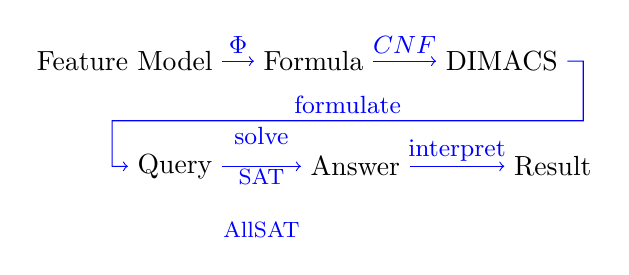
\begin{tikzpicture}
				\tikzset{block/.style={align=center,minimum height=5mm}}
				\node [block] (fm) {Feature Model};
				\node [block, right =4mm of fm] (formula) {Formula};
				\node [block, right =8mm of formula] (cnf) {DIMACS};
				\node [block, below right =8mm and -12mm of fm] (query) {Query};
				\node [block, right =10mm of query] (answer) {Answer};
				\node [block, right =12mm of answer] (result) {Result};
				\node [coordinate, below right =5mm and 2mm of cnf] (right) {};
				\node [coordinate, above left =3mm and 2mm of query] (left) {};
				\path[draw,->,color=blue] (fm) edge node[yshift=2mm] {\small $\Phi$} (formula)
							(formula) edge node[yshift=2mm] {\small $CNF$} (cnf)
							(cnf.east) -| (right) -- node[yshift=2mm] {\small formulate} (left) |- (query)
							(query) edge node[yshift=-2mm,align=center,font={\footnotesize}] {{\small solve}\\[1.5ex]SAT\\\ssat{}\\AllSAT} (answer)
							(answer) edge node [yshift=2mm]{\small interpret} (result);
			\end{tikzpicture}
		\end{definition}
		\begin{note}{}
			for brevity, we assume that $\phi = CNF(\Phi(FM))$ for a given feature model $FM$
		\end{note}
	\end{fancycolumns}
\end{frame}

% TODO I think I need a table here illustrating how the three different solvers can be combined with the three/four queries - to understand what comes next and in which order

\subsection{Consistency, Cardinality, and Enumeration}

\subsubsection{Feature Model}

\begin{frame}{\myframetitle}
	\begin{fancycolumns}[t]
		\emph{Consistency of Feature Models (SAT)}
		\begin{definition}{Void/Consistent Feature Model}
			\begin{itemize}
				\item are there grave modeling errors?
				\item is it possible to configure any product at all?
			\end{itemize}
			\centering
			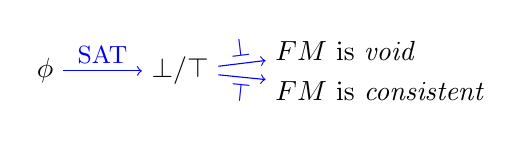
\begin{tikzpicture}
				\tikzset{block/.style={align=center,minimum height=5mm}}
				\node [block] (query) {$\phi$};
				\node [block, right =10mm of query] (answer) {$\bot/\top$};
				\node [block, above right =-3mm and 6mm of answer] (void) {$FM$ is \emph{void}};
				\node [block, below right =-3mm and 6mm of answer] (notvoid) {$FM$ is \emph{consistent}};
				\path[draw,->,color=blue] (query) edge node[yshift=2mm] {\small SAT} (answer)
							(answer) edge node [yshift=2mm,sloped]{\small $\bot$} (void)
							(answer) edge node [yshift=-2mm,sloped]{\small $\top$} (notvoid);
			\end{tikzpicture}
		\end{definition}
		\nextcolumn
		\emph{Cardinality of Feature Models (\ssat{})}
		\begin{definition}{How Many Products Are There?}
			\centering
			\begin{tikzpicture}
				\tikzset{block/.style={align=center,minimum height=5mm}}
				\node [block] (query) {$\phi$};
				\node [block, right =10mm of query] (answer) {$\abs{C}$};
				\path[draw,->,color=blue] (query) edge node[yshift=2mm] {\small \ssat{}} (answer);
			\end{tikzpicture}
		\end{definition}
		\begin{definition}{Variability Factor: Share of Products?}
			\centering
			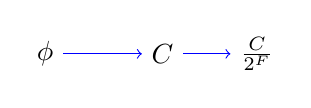
\begin{tikzpicture}
				\tikzset{block/.style={align=center,minimum height=5mm}}
				\node [block] (query) {$\phi$};
				\node [block, right =10mm of query] (answer) {$\abs{C}$};
				\node [block, right =6mm of answer] (num) {$\frac{\abs{C}}{2^{\abs{F}}}$};
				\path[draw,->,color=blue] (query) edge node[yshift=2mm] {\small \ssat{}} (answer)
							(answer) edge node [yshift=2mm,sloped]{} (num);
			\end{tikzpicture}
		\end{definition}
	\end{fancycolumns}
	\begin{fancycolumns}[t]
		\begin{exampletight}{}
			\begin{fancycolumns}[animation=none]
				\centering
				{\small\featureDiagram{Root,concrete[X,concrete,alternative][Y,concrete]}\\$\pnot (X \por Y)$}

				void
			\nextcolumn
				\centering
				{\small\featureDiagram{Root,concrete[X,concrete,alternative][Y,concrete]}\\$X \por Y$}

				consistent
			\end{fancycolumns}
		\end{exampletight}
		\nextcolumn
		\uncover<2->{\begin{exampletight}{}
			\begin{fancycolumns}[animation=none]
				\centering
				{\small\featureDiagram{Root,concrete[X,concrete,alternative][Y,concrete]}\\$\pnot (X \por Y)$}

				$0$ products, VF $0$
			\nextcolumn
				\centering
				{\small\featureDiagram{Root,concrete[X,concrete,alternative][Y,concrete]}\\$X \por Y$}

				$2$ products, VF $\frac{2}{8}$
			\end{fancycolumns}
		\end{exampletight}}
	\end{fancycolumns}
\end{frame}

\begin{frame}{\myframetitle}
	\begin{fancycolumns}[t]
		\emph{Feasibility of SAT-Based Analyses}

		\begin{note}{Is SAT-Based Analysis ``Easy''?}
			\begin{itemize}
				\item provocative claim: \mycite{SAT-based analysis of feature models is easy} \mysource{\href{https://dl.acm.org/doi/10.5555/1753235.1753267}{Mendonca~et~al.~2009}}
				\item easy $=$ performs much better than expected (although NP-complete)
				\item easy $=$ fast?
				\begin{itemize}
					\item what about formulating the query?\\
						(e.g., CNF transformation)
					\item what about many queries?\\
						(e.g., what we discuss next)
				\end{itemize}
			\end{itemize}
		\end{note}
	\nextcolumn
		\emph{Feasibility of \ssat{}-Based Analyses}
	
		\begin{exampletight}{Time to Count Products of Linux}
			\pic[width=\linewidth,page=4]{linux-plots}\\[-3mm]
			\begin{itemize}
				\item the solver from 2023 can solve models from 2003 % TODO which solver?
				\item can we analyze the models from 2023 in 2043?
			\end{itemize}
		\end{exampletight}
	\end{fancycolumns}
\end{frame}


\begin{frame}{\myframetitle}
	\begin{fancycolumns}
		\emph{Enumeration of Feature Models (AllSAT)}
		\begin{definition}{Which Products Are There?}
			\begin{itemize}
				\item \emph{P2(b)}: How to get all products?
			\end{itemize}
			\centering
			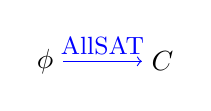
\begin{tikzpicture}
				\tikzset{block/.style={align=center,minimum height=5mm}}
				\node [block] (query) {$\phi$};
				\node [block, right =10mm of query] (answer) {$C$};
				\path[draw,->,color=blue] (query) edge node[yshift=2mm] {\small AllSAT} (answer);
			\end{tikzpicture}
		\end{definition}
		\begin{note}{}
			AllSAT does not scale to realistic feature models!\\
			50 features, configurations \`a 1 Byte $\approx$ 1 Petabyte
		\end{note} % TODO better example? what about the number of features such that it cannot be stored on all servers of the world? or we take a reasonable size of a hard disk in a notebook? 5 terrabyte? I (Thomas) cannot imagine a petabyte.
		\begin{exampletight}{}
			\begin{fancycolumns}[animation=none]
				\centering
				{\small\featureDiagram{Root,concrete[X,concrete,alternative][Y,concrete]}\\$\pnot (X \por Y)$}

				$\varnothing$
			\nextcolumn
				\centering
				{\small\featureDiagram{Root,concrete[X,concrete,alternative][Y,concrete]}\\$X \por Y$}

				$\{\{Root, X\},\{Root, Y\}\}$
			\end{fancycolumns}
		\end{exampletight}
	\nextcolumn
		\centering
		\sffamily
		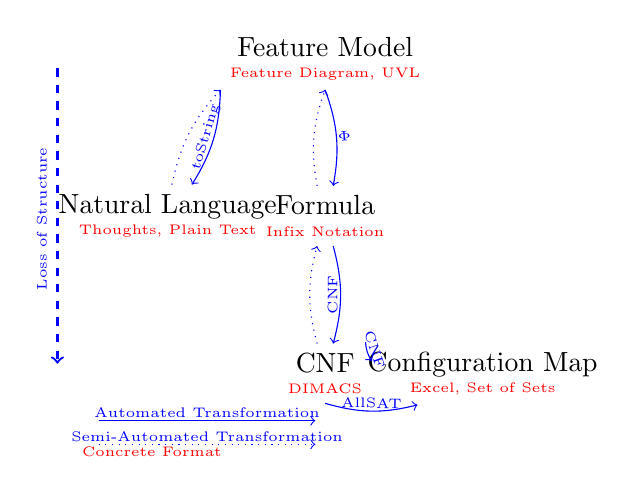
\begin{tikzpicture}
			\tikzstyle{every edge}=[font=\tiny,draw,color=blue]

			\node (topleft) at (-1.4,0) {};
			\node (bottomleft) at (-1.4,-4) {};
			
			\node (fd) at (2,0) [align=center] {Feature Model\\[-1ex]{\tiny\color{red}Feature Diagram, UVL}};
			\node (nat) at (0,-2) [align=center] {Natural Language\\[-1ex]{\tiny\color{red}Thoughts, Plain Text}};
			\node (phi) at (2,-2) [align=center] {Formula\\[-1ex]{\tiny\color{red}Infix Notation}};
			\node (cfg) at (4,-4) [align=center] {Configuration Map\\[-1ex]{\tiny\color{red}Excel, Set of Sets}};
			\node (cnf) at (2,-4) [align=center] {CNF\\[-1ex]{\tiny\color{red}DIMACS}};

			\path [dashed, thick, ->] (topleft) edge node[left, rotate=90, yshift=2mm, xshift=10mm] {Loss of Structure} (bottomleft);
		
			\path [->] (fd.south west) edge[bend left=15] node[sloped,yshift=1mm] {toString} (nat);
			\path [dotted, ->] (nat) edge[bend left=15] node[sloped,yshift=1mm] {} (fd.south west);
			
			\path [->] (fd.south) edge[bend left=15] node[sloped,yshift=1mm,rotate=90] {$\Phi$} (phi);
			\path [dotted, ->] (phi) edge[bend left=15] node[sloped,yshift=2mm,rotate=270] {} (fd.south);

			\path [->] (phi) edge[bend left=15] node[sloped,yshift=1mm] {CNF} (cnf);
			\path [dotted, ->] (cnf) edge[bend left=15] node[sloped,yshift=2mm,rotate=270] {} (phi);
		
			\path [->] (cfg) edge[bend right=15] node[sloped,yshift=1mm] {CNF} (cnf);
			\path [->] (cnf.south) edge[bend right=15] node[sloped,yshift=1mm] {AllSAT} (cfg);

			\node (trans) at (-1,-4.6) {};
			\node (trans2) at (2,-4.6) {};
			\node (trans3) at (-1,-4.9) {};
			\node (trans4) at (2,-4.9) {};
			\path [->] (trans) edge node[yshift=1mm] {Automated Transformation} (trans2);
			\path [dotted, ->] (trans3) edge[yshift=5mm] node[yshift=1mm] {Semi-Automated Transformation} (trans4);
		
			\node (bottomleft2) at (-0.2,-5) {\tiny\color{red}Concrete Format};
		\end{tikzpicture} % TODO position of "Concrete Format" not optimal. gray out irrelevant parts? not sure what to look at here.
	\end{fancycolumns}
\end{frame}

\subsubsection{Features}

\begin{frame}{\myframetitle}
	\begin{fancycolumns}[t]
		\emph{Consistency of Features (SAT)}
		\begin{definition}{Core/Dead Feature}
			\begin{itemize}
				\item can a feature $F$ be (de-)selected at all?
			\end{itemize}
			\centering
			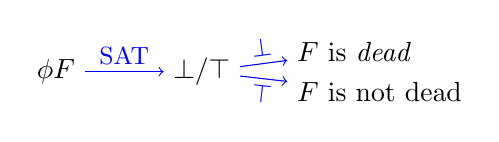
\begin{tikzpicture}
				\tikzset{block/.style={align=center,minimum height=5mm}}
				\node [block] (query) {$\phi \pand F$};
				\node [block, right =10mm of query] (answer) {$\bot/\top$};
				\node [block, above right =-3mm and 6mm of answer] (void) {$F$ is \emph{dead}};
				\node [block, below right =-3mm and 6mm of answer] (notvoid) {$F$ is not dead};
				\path[draw,->,color=blue] (query) edge node[yshift=2mm] {\small SAT} (answer)
							(answer) edge node [yshift=2mm,sloped]{\small $\bot$} (void)
							(answer) edge node [yshift=-2mm,sloped]{\small $\top$} (notvoid);
			\end{tikzpicture}
			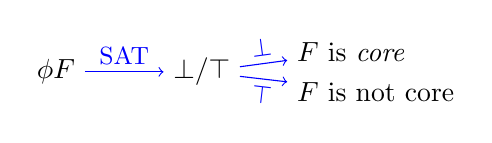
\begin{tikzpicture}
				\tikzset{block/.style={align=center,minimum height=5mm}}
				\node [block] (query) {$\phi \pand \pnot F$};
				\node [block, right =10mm of query] (answer) {$\bot/\top$};
				\node [block, above right =-3mm and 6mm of answer] (void) {$F$ is \emph{core}};
				\node [block, below right =-3mm and 6mm of answer] (notvoid) {$F$ is not core};
				\path[draw,->,color=blue] (query) edge node[yshift=2mm] {\small SAT} (answer)
							(answer) edge node [yshift=2mm,sloped]{\small $\bot$} (void)
							(answer) edge node [yshift=-2mm,sloped]{\small $\top$} (notvoid);
			\end{tikzpicture}
		\end{definition}
		\nextcolumn
		\emph{Cardinality of Features (\ssat{})}
		\begin{definition}{How Many Products Include Feature $F$?}
			\centering
			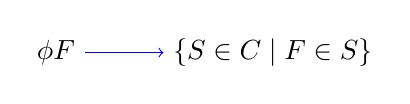
\begin{tikzpicture}
				\tikzset{block/.style={align=center,minimum height=5mm}}
				\node [block] (query) {$\phi \pand F$};
				\node [block, right =10mm of query] (answer) {$\abs{\{S \in C \mid F \in S\}}$};
				\path[draw,->,color=blue] (query) edge node[yshift=2mm] {\small \ssat{}} (answer);
			\end{tikzpicture}
		\end{definition}
		\begin{definition}{Commonality: How Constrained is This Feature?}
			\centering
			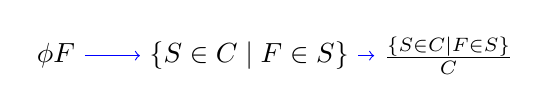
\begin{tikzpicture}
				\tikzset{block/.style={align=center,minimum height=5mm}}
				\node [block] (query) {$\phi \pand F$};
				\node [block, right =7mm of query] (answer) {$\abs{\{S \in C \mid F \in S\}}$};
				\node [block, right =2mm of answer] (num) {$\frac{\abs{\{S \in C \mid F \in S\}}}{\abs{C}}$};
				\path[draw,->,color=blue] (query) edge node[yshift=2mm] {\small \ssat{}} (answer)
							(answer) edge node [yshift=2mm,sloped]{} (num);
			\end{tikzpicture}
		\end{definition}
	\end{fancycolumns}
	\begin{fancycolumns}[t]
		\begin{exampletight}{}
			\centering
			{\small\featureDiagram{Root,concrete[X,concrete,alternative][Y,concrete]}\\$\pnot X$}

			$X$ is dead\hfill$Root$ and $Y$ are core
		\end{exampletight}
		\nextcolumn
		\begin{exampletight}{}
			\centering
			{\small\featureDiagram{Root,concrete[X,concrete,alternative][Y,concrete]}\\$\pnot X$}

			$X$: 0 products\hfill$Root$ and $Y$: 1 products
		\end{exampletight}
	\end{fancycolumns}
\end{frame}

\subsubsection{Partial Configurations}

\begin{frame}{\myframetitle}
	\begin{fancycolumns}[t]
		\emph{Consistency of Partial Configurations (SAT)}
		\begin{definition}{Valid Partial Configuration}
			Is a partial configuration $C = ({\color{green}S}, {\color{red}D})$ consistent with the feature model? % TODO would be easier if term valid could be used here

			\centering
			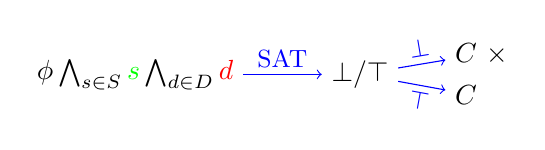
\begin{tikzpicture}
				\tikzset{block/.style={align=center,minimum height=5mm}}
				\node [block] (query) {$\phi \pand \bigwedge_{s \in S} {\color{green}s} \pand \bigwedge_{d \in D} {\color{red}\pnot d}$};
				\node [block, right =10mm of query] (answer) {$\bot/\top$};
				\node [block, above right =-3mm and 6mm of answer] (void) {$C$ $\times$};
				\node [block, below right =-3mm and 6mm of answer] (notvoid) {$C$ \checkmark};
				\path[draw,->,color=blue] (query) edge node[yshift=2mm] {\small SAT} (answer)
							(answer) edge node [yshift=2mm,sloped]{\small $\bot$} (void)
							(answer) edge node [yshift=-2mm,sloped]{\small $\top$} (notvoid);
			\end{tikzpicture}
		\end{definition}
		\nextcolumn
		\emph{Cardinality of Partial Configurations (\ssat{})}
		\begin{definition}{How Many Products Are Still Configurable for $C$?}
			\centering
			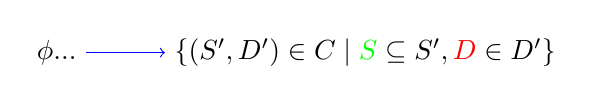
\begin{tikzpicture}
				\tikzset{block/.style={align=center,minimum height=5mm}}
				\node [block] (query) {$\phi \pand ...$};
				\node [block, right =10mm of query] (answer) {$\abs{\{(S', D') \in C \mid {\color{green}S} \subseteq S', {\color{red}D} \in D'\}}$};
				\path[draw,->,color=blue] (query) edge node[yshift=2mm] {\small \ssat{}} (answer);
			\end{tikzpicture}
		\end{definition}
	\end{fancycolumns}
	\begin{fancycolumns}[t]
		\begin{exampletight}{}
			\centering
			{\small\featureDiagram{Root,concrete[X,concrete,optional][Y,concrete,optional]}\\$X \pimplies Y$}

			\cfg{Root}{X} \checkmark
		\end{exampletight}
		\nextcolumn
		\begin{exampletight}{}
			\centering
			{\small\featureDiagram{Root,concrete[X,concrete,optional][Y,concrete,optional]}\\$X \pimplies Y$}

			\cfg{Root}{X}: 2 products
		\end{exampletight}
	\end{fancycolumns}
\end{frame}

\subsection{Automated Analyses in FeatureIDE}

\subsubsection*{Feature-Model Editor}

\begin{frame}{\myframetitle}
	\begin{fancycolumns}[widths={60,40}]
		\begin{exampletight}{} % TODO would be great to show an explanation here
			\picDark[width=\textwidth]{featureide-feature-model-editor-waffle}
		\end{exampletight}
	\nextcolumn
		\begin{exampletight}{}
			\picDark[width=\textwidth]{featureide-feature-model-statistics}
		\end{exampletight}
	\end{fancycolumns}
\end{frame}

\subsubsection*{Configuration Editor}

\begin{frame}{\myframetitle}
	\begin{fancycolumns}[widths={60,40}]
		\begin{exampletight}{}
			\centering
			\picDark[width=.27\textwidth]{featureide-configuration-editor-step1}
			$\Rightarrow$
			\picDark[width=.63\textwidth]{featureide-configuration-editor-step2}
		\end{exampletight}
	\nextcolumn
		\begin{note}{Decision Propagation}
			\begin{itemize}
				\item after each decision (i.e., click) \ldots
				\begin{itemize}
					\item \ldots{} select features that are now \emph{conditionally core}
					\item \ldots{} deselect features that are now \emph{conditionally dead}
				\end{itemize}
				\item this way it is impossible to configure an invalid configuration
				\item explanations for all propagated decisions
			\end{itemize}
		\end{note}
	\end{fancycolumns}
\end{frame}

\begin{frame}{Automated Analysis of Feature Models}
	\begin{fancycolumns}
		\begin{definition}{The Road So Far \ldots}
			\centering
			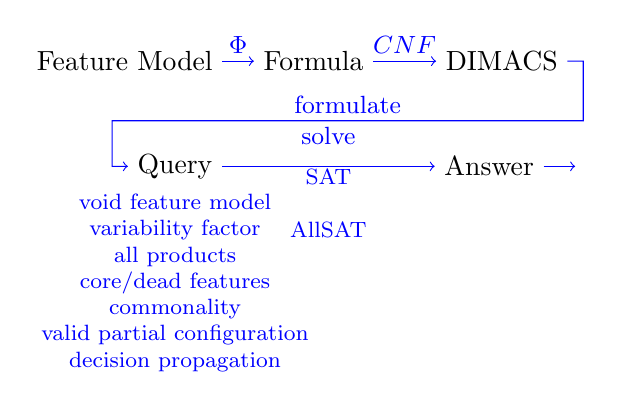
\begin{tikzpicture}
				\tikzset{block/.style={align=center,minimum height=5mm}}
				\node [block] (fm) {Feature Model};
				\node [block, right =4mm of fm] (formula) {Formula};
				\node [block, right =8mm of formula] (cnf) {DIMACS};
				\node [block, below right =8mm and -12mm of fm] (query) {Query};
				\node [block, below =-.5mm of query,align=center,color=blue,font={\footnotesize}] (query2) {void feature model\\variability factor\\all products\\core/dead features\\commonality\\valid partial configuration\\decision propagation};
				\node [block, right =27mm of query] (answer) {Answer};
				\node [block, right =4mm of answer] (result) {};
				\node [coordinate, below right =5mm and 2mm of cnf] (right) {};
				\node [coordinate, above left =3mm and 2mm of query] (left) {};
				\path[draw,->,color=blue] (fm) edge node[yshift=2mm] {\small $\Phi$} (formula)
							(formula) edge node[yshift=2mm,align=center] {\small $CNF$} (cnf)
							(cnf.east) -| (right) -- node[yshift=2mm] {\small formulate} (left) |- (query)
							(query) edge node[yshift=-2mm,align=center,font={\footnotesize}] {{\small solve}\\[1.5ex]SAT\\\ssat{}\\AllSAT} (answer)
							(answer) edge (result);
			\end{tikzpicture}
		\end{definition}
	\nextcolumn
		\begin{definition}{\ldots\ and Beyond}
			\centering
			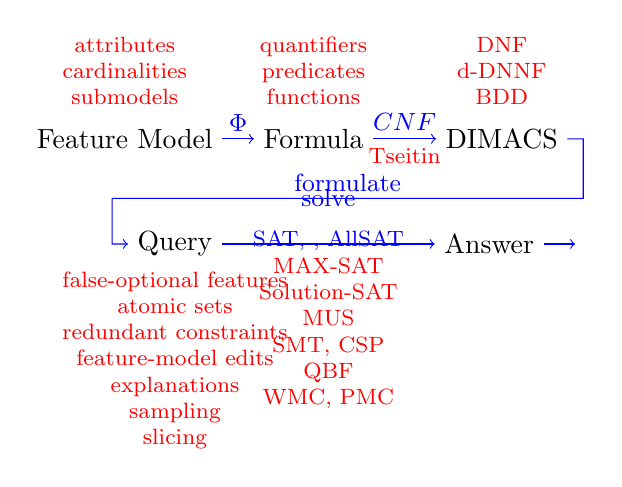
\begin{tikzpicture}
				\tikzset{block/.style={align=center,minimum height=5mm}}
				\node [block,align=center,color=red,font={\footnotesize}] (fm2) {attributes\\cardinalities\\submodels};
				\node [block, below =.5mm of fm2] (fm) {Feature Model};
				\node [block, right =4mm of fm] (formula) {Formula};
				\node [block, above =.5mm of formula,align=center,color=red,font={\footnotesize}] (formula2) {quantifiers\\predicates\\functions};
				\node [block, right =8mm of formula] (cnf) {DIMACS};
				\node [block, above =.5mm of cnf,align=center,color=red,font={\footnotesize}] (cnf2) {DNF\\d-DNNF\\BDD};
				\node [block, below right =8mm and -12mm of fm] (query) {Query};
				\node [block, below =-.5mm of query,align=center,color=red,font={\footnotesize}] (query2) {false-optional features\\atomic sets\\redundant constraints\\feature-model edits\\explanations\\sampling\\slicing};
				\node [block, right =27mm of query] (answer) {Answer};
				\node [block, right =4mm of answer] (result) {};
				\node [coordinate, below right =5mm and 2mm of cnf] (right) {};
				\node [coordinate, above left =3mm and 2mm of query] (left) {};
				\path[draw,->,color=blue] (fm) edge node[yshift=2mm] {\small $\Phi$} (formula)
							(formula) edge node[yshift=0mm,align=center] {\small $CNF$\\{\footnotesize\color{red}Tseitin}} (cnf)
							(cnf.east) -| (right) -- node[yshift=2mm] {\small formulate} (left) |- (query)
							(query) edge node[yshift=-7mm,align=center,font={\footnotesize}] {{\small solve}\\[1.5ex]SAT, \ssat{}, AllSAT\\{\color{red}MAX-SAT}\\{\color{red}Solution-SAT}\\{\color{red}MUS}\\{\color{red}SMT, CSP}\\{\color{red}QBF}\\{\color{red}WMC, PMC}} (answer)
							(answer) edge (result);
			\end{tikzpicture}
			\vspace*{-3ex}
			\begin{itemize}
				\item develop new analyses
				\item improve efficiency of existing analyses
				\item investigate correctness and compositionality
			\end{itemize}
		\end{definition}
	\end{fancycolumns}
\end{frame}